% Created 2022-01-30 Sun 09:50
% Intended LaTeX compiler: xelatex
\documentclass[11pt,twoside,landscape]{article}
\usepackage{graphicx}
\usepackage{longtable}
\usepackage{wrapfig}
\usepackage{rotating}
\usepackage[normalem]{ulem}
\usepackage{amsmath}
\usepackage{amssymb}
\usepackage{capt-of}
\usepackage{hyperref}
\usepackage[newfloat]{minted}
\usepackage{color}
\usepackage{listings}
\usepackage[top=2cm,bottom=2cm,right=2cm,left=2cm,landscape]{geometry}
\usepackage{multicol}
\usepackage{enumitem}
\usepackage{fancyhdr}
\setlist{noitemsep}
\setlength{\parindent}{0pt}
\setlength{\columnseprule}{0.2pt}
\definecolor{mygreen}{rgb}{0,0.6,0}
\definecolor{mygray}{rgb}{0.5,0.5,0.5}
\definecolor{mymauve}{rgb}{0.58,0,0.82}
\lstset{ backgroundcolor=\color{white}, basicstyle=\footnotesize, breaklines=true, captionpos=b, commentstyle=\color{mygreen}, escapeinside={\%*}{*)},keywordstyle=\color{blue}, stringstyle=\color{mymauve},}
\usepackage{caption}
\author{Olivier Lischer}
\date{\today}
\title{CPl Summary}
\hypersetup{
 pdfauthor={Olivier Lischer},
 pdftitle={CPl Summary},
 pdfkeywords={},
 pdfsubject={},
 pdfcreator={Emacs 27.2 (Org mode 9.5.2)}, 
 pdflang={English}}
\begin{document}

\pagestyle{fancy}
\fancyhf{}
\fancyhead[R]{CPl-HS21}
\fancyhead[L]{Exam Summary}
\fancyfoot[CE,CO]{\leftmark}
\fancyfoot[R]{\thepage}
\fancyfoot[L]{Olivier Lischer}

\tableofcontents
\newpage
\begin{multicols}{3}

\section{General}
\label{sec:orgffac35d}
\textbf{Compilation Process}

The C++ Compilation process consits of 3 steps:
\begin{enumerate}
\item Preprocessor (textual replacement in the files and execution of the \texttt{\#}-strings
\item Compiler (compile each *.cpp file in to object code)
\item Linker (link all object code files to a library / executable / \ldots{}
\end{enumerate}


\textbf{Best Practice Setup}

A modern \href{../../../roam/20210920103243-c.org}{C++} project is divided in 3 subprojects:
\begin{itemize}
\item library: the whole application logic
\item testing: project for \href{../../../roam/20210920103754-unit_testing.org}{Unit Testing} (for example with \href{../../../roam/20210920103820-cute.org}{CUTE})
\item executable: small project with only a main function which calls the entrypoint in the library
\end{itemize}


\textbf{Decleration / Definition}

In \href{../../../roam/20210920103243-c.org}{C++} everything has to be declared before they can be used.
Declarations are normally written in .h files.
Multiple declaration for the same thing is sometimes allowed for example for functions.
An example for a definition: \texttt{void sayHello(std::ostream \&out);}

The definition is normally written in a .cpp file and contains the actual code.
Each definition can only occure once.
This is also called \href{../../../roam/20210920104915-one_definition_rule.org}{One Definition Rule}.
Example for a declaration: \texttt{void sayHello(std::ostream \&out) \{ /* Body */ \}}

\textbf{ODR / One Definition Rule}

In \href{../../../roam/20210920103243-c.org}{C++} everything can only have one definition.
This is called the \emph{One Definition Rule}.

\textbf{Include Guards}

In \href{../../../roam/20210920103243-c.org}{C++} declerations are included over the \texttt{\#include} keyword.
To prevent recursive includes the following code snippets is used.
This is called \emph{Include guard}:
\lstset{language=c++,label= ,caption= ,captionpos=b,numbers=none}
\begin{lstlisting}
#ifndef SAYHELLO_H_
#define SAYHELLO_H_
/* content */
#endif /* SAYHELLO_H_ */
\end{lstlisting}

Some compiler have the keyword \texttt{\#pragma once}.
This should not be used because it is not standard C++.

\textbf{Value Semantic}

\href{../../../roam/20210920103243-c.org}{C++} has a default value semantic.
That means that every object is normally copied.
In \href{../../../roam/20201116150053-java.org}{Java} normally only the Reference to the object is copied.

\textbf{References}

In \href{../../../roam/20210920103243-c.org}{C++} references are not the same as in Java.
References in C++ are just another name for a existing object.
In a local context this is not useful.
Used as parameters in function they can be very useful:

\begin{itemize}
\item \texttt{void scale(Point point)}: No side-effect (call by value)
\item \texttt{void scale(Point \& point)}: Has side-effect (call by ref)
\end{itemize}


\textbf{Casting}

In modern \href{../../../roam/20210920103243-c.org}{CPP} you use normally the \texttt{static\_cast} operator.

\lstset{language=c++,label= ,caption= ,captionpos=b,numbers=none}
\begin{lstlisting}
enum class Month {
  Jan = 1, Feb, Mar, Apr, May, Jun, Jul, Aug, Sep, Oct, Nov, Dec
};

Month fromIntToMonth(int month) {
  if (month < 1 && month > 12) {
    throw std::invalid_argument{"moth must be between 1 and 12"};
  }

  return static_cast<Month>(month);
}
\end{lstlisting}

\textbf{Variable Definition}

In modern \href{../../../roam/20210920103243-c.org}{CPP} you should use the \texttt{\{\}} syntax to initialize new variables:
\lstset{language=c++,label= ,caption= ,captionpos=b,numbers=none}
\begin{lstlisting}
int anAnswer{42}; int zero{};
\end{lstlisting}

When you use the keyword \texttt{auto} (use it!) then the equal sign (\texttt{=}) should be used:
\lstset{language=c++,label= ,caption= ,captionpos=b,numbers=none}
\begin{lstlisting}
auto someType = 4;
\end{lstlisting}

\textbf{Bit wise operations}

When working with bit wise operations only unsigned integers should be used.
Because the first bit in a signed integer indicates if it is a positive or negative number

\textbf{Strings}

In \href{../../../roam/20210920103243-c.org}{CPP} exits two kinds of strings, the \href{../../../roam/20211008113512-c.org}{C} style strings and the \texttt{std::string}.
The C style should not be used anymore (when possible).
A big different between \href{../../../roam/20201116150053-java.org}{Java} and \href{../../../roam/20211003114158-c.org}{C\#} is that the string in \href{../../../roam/20210920103243-c.org}{CPP} are mutable. 

For each kind of string exits a string literal:
\begin{itemize}
\item \texttt{"ab"} is an array of const chars (is immutable)
\item \texttt{"ab"s} is an std::string
\begin{itemize}
\item this requires \texttt{using namespace std::literals;}
\item this is sometimes used with \texttt{auto}
\end{itemize}
\end{itemize}


\textbf{Input Streams}

\texttt{std::cin} represents STDIN.
When using \texttt{std::cin} with the \texttt{>>} operator it skips all kinds of white spaces.
With \texttt{std::cin.get()} the white spaces are not skipped.
The chars on a input stream ore only consumed if the reading was successfully.
If does a read fail it goes in a fail state and all subsequent read fail as well.
Before reading from a input stream object you should always check its state.


\lstset{language=c++,label= ,caption= ,captionpos=b,numbers=none}
\begin{lstlisting}
int inputAge(std::istream & in) {
  std::string line{};
  while (getline(in, line)) {
    std::istringstream is{line};
    int age{-1};
    if (is >> age) {
      return age;
    }
  }
  return -1;
}
\end{lstlisting}

\textbf{Output Stream}

The \texttt{std::cout} it the STDOUT.
For modifying the behavior of the output stream so called \href{../../../roam/20211008115905-manipulators_in_cpp.org}{Manipulators} can be used.

\textbf{Output Manipulators}

The manipulators for output stream are defined in \texttt{<ios>} and \texttt{<iomanip>}

{
\begin{center}
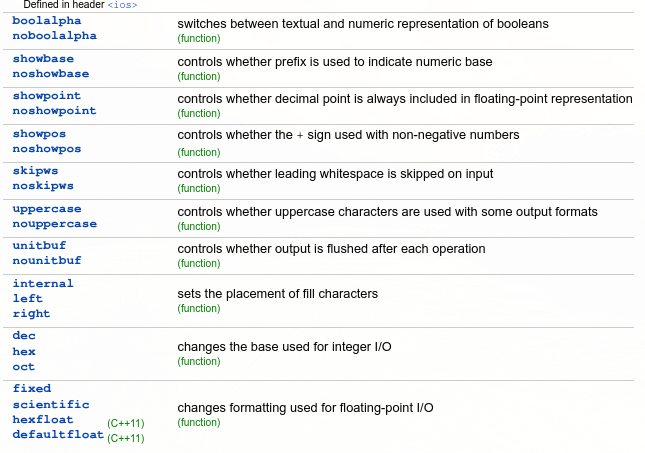
\includegraphics[width=.9\linewidth]{img/manipulator.png}
\end{center}
\captionof{figure}{Manipulators}
}

\textbf{IO in CPP}

The header files for IO are:
\begin{itemize}
\item \emph{<iosfwd>} contains only declarations
\item \emph{<istream>} contains input implementation
\item \emph{<ostream>} contains output implementation
\item \emph{<iostream>} contains all of the previous inkl. \texttt{std::cout}, \texttt{std::in}, \texttt{std::cerr} (should only used in main)
\end{itemize}


\textbf{Type Aliases}

Using type aliases a long and complicated type could be asigned a shorter name.
\texttt{using <alias-name> = <type>;}

\lstset{language=c++,label= ,caption= ,captionpos=b,numbers=none}
\begin{lstlisting}
using input = std::istream_iterator<std:::string>;
input eof{}; // defult std::istream_iterator is EOF
input in{std::cin};
std::ostream_iterator<std::string> out{std::cout, " "};
std::copy(in, eof, out);
\end{lstlisting}

\textbf{When you should use references, when values}

As a rule of thumb when to use \href{../../../roam/20210920111001-c_references.org}{C++ References} go with the following:

\begin{enumerate}
\item value parameter - default
\item reference parameter - when side-effect is required at call side
\item const reference parameter - when type is large and no side-effects desired at call-site
\item const value parameter - just coding style, can prevent changing the parameter inside the function inadvertently (de. versehentlich)
\end{enumerate}

\textbf{When you should return references, when values}

As a rule of thumb when to return \href{../../../roam/20210920111001-c_references.org}{C++ References}
\begin{enumerate}
\item value - default
\item reference
\begin{itemize}
\item return only a reference parameter or from a member function a member variable
\item \textbf{Never return a reference to a local variable!} (Undefined behavior)
\end{itemize}
\item by const value
\begin{itemize}
\item \textbf{Do not do this}. It just annoys the caller
\end{itemize}
\end{enumerate}

\textbf{auto as return value}

The \texttt{auto} keyword can be used as a return type. If \texttt{auto} is specified then the return value is deduced from return statements. You can also specify the return type with \texttt{auto} and append a \texttt{->} at the end with the return value. This is often used to align all function names.

\lstset{language=c++,label= ,caption= ,captionpos=b,numbers=none}
\begin{lstlisting}
auto middle(std::vector<int> const & c) -> int;
auto middle(std::vector<int> const & c) -> int {
  if (c.size() == 0) { throw new invalid_argument{}; }
  return c[c.size() / 2];
}
\end{lstlisting}

\textbf{Default Arguments}

\lstset{language=c++,label= ,caption= ,captionpos=b,numbers=none}
\begin{lstlisting}
// incr.h
void incr(int &var, unsigned delta = 1);

// incr.cpp
void incr(int &var, unsigned delta) {
  var += delta;
}
\end{lstlisting}

Default parameters can only be written at the end.
Implicit overload of the function with fewer parameters.
Default arguments can be omitted when calling the function.

\textbf{Functions as parameters}

\lstset{language=c++,label= ,caption= ,captionpos=b,numbers=none}
\begin{lstlisting}
void applyAndPrint(double x, double f(double)) {
  std::cout << "f" << x << ") = " << f(x) << '\n';
}

void applyAndPrint(double x, double (&f)(double)) {
  std::cout << "f" << x << ") = " << f(x) << '\n';
}

void applayAndPrint(double x, std::function<double(double)> f) { // recomended
  f(x);
}
\end{lstlisting}

A function parameter declared like \texttt{double f(double)} does not accept a lambda with a capture.
Instead you should use \texttt{std::function<double(double)> f} this could be used for lambdas with captures.
This is also the recommended way.

{
\begin{center}
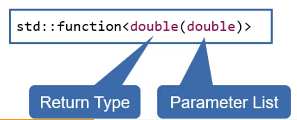
\includegraphics[width=.9\linewidth]{img/std_function.png}
\end{center}
\captionof{figure}{std::function example}
}


\textbf{Lambdas with capture}

If you want to assign a lambda to a variable you must use the \texttt{auto} keyword. Only the compiler knows the real type. 
In lambdas the parameter list can only omitted when the return type is not specified.

capturing a local variable by value:
\lstset{language=c++,label= ,caption= ,captionpos=b,numbers=none}
\begin{lstlisting}
int x = 5;
auto l = [x]() mutable {
  std::cout << ++x;
 };
\end{lstlisting}

capturing a local variable by ref:
\lstset{language=c++,label= ,caption= ,captionpos=b,numbers=none}
\begin{lstlisting}
int x = 5;
auto const l = [&x]() {
  std::cout << ++x;
 }; 
\end{lstlisting}

capturing all local variables by value:
\lstset{language=c++,label= ,caption= ,captionpos=b,numbers=none}
\begin{lstlisting}
int x = 5;
auto l = [=]() mutable {
  std::cout << ++x;
 };
\end{lstlisting}

capturing all local variables by ref:
\lstset{language=c++,label= ,caption= ,captionpos=b,numbers=none}
\begin{lstlisting}
auto l = [&]() mutable {
  std::cout << ++x;
 };
\end{lstlisting}

\texttt{this} can be also captured


\lstset{language=c++,label= ,caption= ,captionpos=b,numbers=none}
\begin{lstlisting}
auto squares = [x=1]() mutable {
  std::cout << x *= 2;
};
\end{lstlisting}
\texttt{x} is \texttt{auto} and is stored for all lambda calls (2, 4, 8, 16, \ldots{})

\textbf{Exceptions}

In \href{../../../roam/20210920103243-c.org}{CPP} any copyable type can be thrown but you should only throw exception
You do not need the \emph{new} keyword. This would throw a pointer of an exception.
\lstset{language=c++,label= ,caption= ,captionpos=b,numbers=none}
\begin{lstlisting}
throw std::invalid_argument{"Description"};
\end{lstlisting}

In an Exception are no meta information available. 


In \href{../../../roam/20210920103243-c.org}{CPP} you have only \texttt{try} and \texttt{catch}. \texttt{finally} does not exists.
The principle is throw by value, catch be \texttt{const} reference.
This avoids unnecessary coping and allows dynamic polymorphism for class types.

The sequence of catches is significant because the first match wins.
To catch all you can use the ellipsis \texttt{(...)}.
This must be the last catch otherwise the later catches would never be executed.

To rethrow an exception just throw it again.

\lstset{language=c++,label= ,caption= ,captionpos=b,numbers=none}
\begin{lstlisting}
try {
  f("do something");
}
catch (std::invalid_argument const &c) {
  // do something
}
catch (...) {
  // catch all 
}
\end{lstlisting}

\textbf{Undefined Behaviour in Call Sequence}

It is not defined in which order the function are evaluated.
It could be that the first \texttt{inputName} and then the seconds is processed.
It could be also the other way be.
If you are not sure use variables to store the output of the function and use the variable as argument for the function call.
\lstset{language=c++,label= ,caption= ,captionpos=b,numbers=none}
\begin{lstlisting}
sayGreeting(std::cout,
	    inputName(std::cin),
	    inputName(std::cin));
\end{lstlisting}

\section{STL Containers}
\label{sec:orgee2d17c}
\subsection{Sequence Containers}
\label{sec:org12d03b5}
\textbf{Sequence Containers}

All elements are accessible in the same order as they were inserted.
To find an element in the container linear time (\(O(n))\) is needed.

\begin{itemize}
\item \texttt{std::vector<T>} in \texttt{<vector>}
\item \texttt{std::deque<T>} in \texttt{<deque>}
\item \texttt{std::list<T> (double linked list)} in \texttt{<list>}
\item \texttt{std::forward\_list<T> (single list)} in \texttt{<forward\_list>}
\item \texttt{std::array<N, T>} in \texttt{<array>}
\end{itemize}


\emph{Attention:} Both list has \emph{NO} index access.

When you use sequence containers in CPP you should normally use the \texttt{std::vector} or the \texttt{std::deque} because they are very efficient.
Except you use it in a bad way.

\textbf{Array}

\href{../../../roam/20210920103243-c.org}{CPP} has two types of arrays:
\begin{itemize}
\item plain C-Arrays (should not be used)
\item \texttt{std::array} (defined in \texttt{<array>})
\end{itemize}

When you need arrays always use \texttt{std::array} instead of the C style arrays.
For \texttt{std::array} you do not need to handle raw pointers.
Additional \texttt{std::array} has some convenient features like storing the length of the array.


The size has to be known at compile time.
\lstset{language=c++,label= ,caption= ,captionpos=b,numbers=none}
\begin{lstlisting}
std::array<int, 5> name{1, 2, 3, 4, 5};
\end{lstlisting}



The std::array has two possibles to access the elements inside:
\begin{itemize}
\item using the \texttt{at()} function, this throws an exception on invalid index access
\item using the \texttt{[]} operation, this has undefined behavior on invalid index access
\end{itemize}


\textbf{vector}

The vector in \href{../../../roam/20210920103243-c.org}{CPP} is a dynamic sized container.
To use it the header file \texttt{<vector>} needs to be included.
The elements can be access with \texttt{at()} and \texttt{[]}.
To insert a new element at the end the function \texttt{push\_back()} is used.
Also the function \texttt{insert()} exists to insert an element somewhere in the vector.

\lstset{language=c++,label= ,caption= ,captionpos=b,numbers=none}
\begin{lstlisting}
std::vector<int> v{};
v.push_back(2);
auto it = v.begin();
v.insert(it, 3);
\end{lstlisting}

\textbf{Sequence Adapters in STL}

In the std library exits LIFO and FIFO Adapters for the sequence containers.
They are based on a real / full container.
But they implement only the required functions.

LIFO Adapter:
\begin{itemize}
\item \texttt{std::stack} in \texttt{<stack>}
\end{itemize}

FIFO Adapter:
\begin{itemize}
\item \texttt{std::queue} in \texttt{<queue>}
\end{itemize}


The \texttt{std::priority\_queue} is also just an adapter.

\subsection{Associative Containers}
\label{sec:org159ef95}
\textbf{Associative Containers}

The elements in an Associative Container are \textbf{always} stored in sorted order.
Because of that the \texttt{find()} member method runs in logarithmic time.
So you should always use the \texttt{find()} method of the member itself.


\begin{itemize}
\item \texttt{std::set<T>} in \texttt{<set>}
\item \texttt{std::multiset<T>} in \texttt{<set>}
\item \texttt{std::map<K, V>} in \texttt{<map>}
\item \texttt{std::multimap<K, V>} in \texttt{<map>}
\end{itemize}


These containers allow the use of functors to manipulate how the data should be stored.

\lstset{language=c++,label= ,caption= ,captionpos=b,numbers=none}
\begin{lstlisting}
#include <set>
#include <functional>

int main() {
  std::set<int, std::greater<>> reverse_int_set{};
}
\end{lstlisting}

\textbf{Set}

You can not modify the elements inside the set.
This could break the order inside the data structure.

You use \texttt{.find()} / \texttt{.count()} member function because it is a lot faster.
\texttt{.count(element)} will return 0 or 1.
To check if the set contains an element use \texttt{.count(element) =} 1=

\textbf{Map}

The iterator access returns a \texttt{std::pair<key, value>}.
The index operator inserts a \emph{new} entry automatically if the key is not availabel.

To check if the set contains an element use \texttt{.count(element) =} 1=

\textbf{Multiset}

The multiset has three special member functions:
\begin{itemize}
\item \texttt{equal\_range()}: returns a range (\texttt{std::pair}) containing all elements with the given key in the container
\item \texttt{lower\_bound()}: returns an iterator pointing to the first element that is \emph{not less} than the key.
\item \texttt{upper\_bound()}: returns an iterator pointing to the first element that is \emph{greater} than the key.
\end{itemize}


\textbf{Multimap}

The multimap has three special member functions:
\begin{itemize}
\item \texttt{equal\_range()}: returns a range (\texttt{std::pair}) containing all elements with the given key in the container
\item \texttt{lower\_bound()}: returns an iterator pointing to the first element that is \textbf{not less} than the key.
\item \texttt{upper\_bound()}: returns an iterator pointing to the first element that is \textbf{greater} than the key.
\end{itemize}

\subsection{Hashed Containers}
\label{sec:org9687063}

The elements in a Hashed Container are stored in an unspecified order.
The \texttt{.find()} member function runs in constant time (\$O(1)).
Therefore, you should use the member function to find elements inside a hashed container


\begin{itemize}
\item \texttt{std::unordered\_set} in \texttt{<unordered\_set>}
\item \texttt{std::unordered\_map} in \texttt{<unordered\_map>}
\end{itemize}


Implementing your own Hash Function is hard and prone to failures.
Stick to standard types like \texttt{std::string} for the keys.

\subsection{Iterators}
\label{sec:org1157f0e}
\textbf{Iterator Kinds}
In CPP exits two kinds of iterators:
\begin{itemize}
\item input iterator
\item forward iterator
\item bidirectional iterator
\item random access iterator
\item output iterator
\end{itemize}


{
\begin{center}
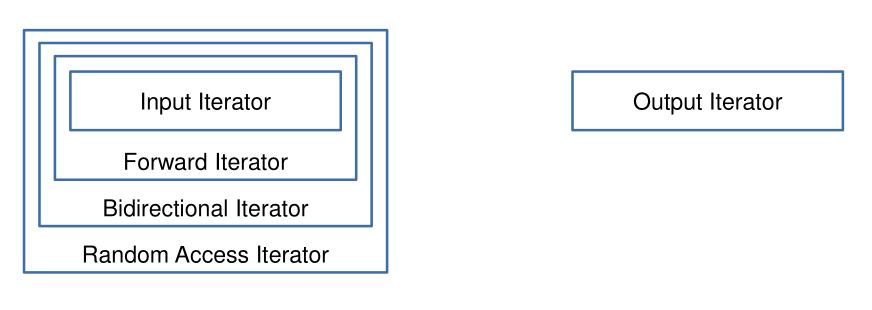
\includegraphics[width=.9\linewidth]{img/stl_iterator_categories.png}
\end{center}
\captionof{figure}{STL Iterator Categories}
}

\textbf{Input Iterator}

The input iterator can only go in one direction and can only read.
The iterator can be copied.
But after an increment all other copies are invalid.
But \texttt{*it++} is explicit allowed by the standard.

\textbf{Forward Iterator}

The forward iterator can do whatever an input iterator can.
Additional it can:
\begin{itemize}
\item changing the "current" element (as long the container / element are not const)
\item the iterator copy can be kept for later references
\end{itemize}

\textbf{Bidirectional Iterator}

The bidirectional iterator can do whatever the forward iterator can do.
Additional it can:
\begin{itemize}
\item go backwards (\texttt{it-{}-})
\end{itemize}

\textbf{Random Access Iterator}

The random access iterator can do whatever the bidirectional iterator can do.
Additional it can:
\begin{itemize}
\item directly access elements at index (positive / negative)
\item go \(n\) steps forward / backwards
\item subtract two iterators to get the distance
\item compare with relational operators (\texttt{<}, \texttt{<=}, \texttt{>}, \texttt{>=})
\end{itemize}


\textbf{Output Iterator}

The output iterator can only write a value to the current element.
But this is only possible once (\texttt{*it=value}).
After that the iterator has to be incremented (\texttt{it++}).
The output iterator has not end-iterator. 

Most other iterators can act also as an output iterator.
Except the underlying container is \texttt{const}.
The Associative Containers are an exception because they return only a read-only iterator.

\textbf{Stream Iterator}

Streams can not be used directly with the algorithms from the standard library.
I have to create an iterator for a stream:
\lstset{language=c++,label= ,caption= ,captionpos=b,numbers=none}
\begin{lstlisting}
std::ostream_iterator<int>{std::cout, ", "}
std::istream_iterator<int>{std::cin, ", "}
\end{lstlisting}

The output stream iterator (\texttt{ostream\_iterator}) does not have an \texttt{end()} marker (theoretically you can print forever on this stream).
With this stream iterators type aliases are interesting.

The default constructed \texttt{std::istream\_iterator<T>} marks the EOF.
Normally an \texttt{istream\_iterator} uses the \texttt{>>} operator for input.
Only the \texttt{std::istreambuf\_iterator<char>} uses the \texttt{std::istream::get()} function.

\lstset{language=c++,label= ,caption= ,captionpos=b,numbers=none}
\begin{lstlisting}
#include <sstream>
#include <iterator>
#include <algorithms>

int main() {
  std::istringstream str2("1 3 5 7 8 9 10");
  auto it = std::find_if(std::istream_iterator<int>(str2),
			 std::istream_iterator<int>(), // EOF
			 [](int i){return i%2 == 0;});
}
\end{lstlisting}

\textbf{const\textsubscript{iterator} vs const iterator}

If you declare an iterator as \texttt{const} (\texttt{const auto it}) you are not allowed to modify the iterator itself.
Therefore, you can not increment the iterator (\texttt{it++}).
Normally this is not what you want.

The const\textsubscript{iterator} itself is \emph{NOT} \texttt{const}.
But the underlying element is \texttt{const} and can not be modified.
The functions \texttt{cbegin()} and \texttt{cend()} return such an iterator.

\textbf{Iterators for inserting}

If you use an iterator to specifying the output for an algorithm you need to make sure that enough space is allocated. 
For this you could use the following functions to create an iterator:
\begin{itemize}
\item \texttt{std::back\_inserter}: creates an iterator which uses the \texttt{push\_back} member function
\item \texttt{std::front\_inserter}: creates an iterator which uses the \texttt{push\_front} member function
\item \texttt{inserter}: creates an iterator which uses the \texttt{insert} member function
\end{itemize}

\section{Algorithms}
\label{sec:orgd3231c3}
\textbf{Why should you use STL algorithm}

Writing your own algorithms, especial loops, is error-prone. 
Additional it is difficult to read and understand what your code does.
Also, the algorithms in the STL are often faster than your own algorithms.

\textbf{algorithms}

The \href{../../../roam/20210920103243-c.org}{CPP} standard library offers us a lot of algorithms.
All of them take iterators as an argument to iterate over the containers. 

The algorithms are defined in:
\begin{itemize}
\item \texttt{<algorithm>}: \texttt{std::count}, \texttt{std::for\_each}, \ldots{}
\item \texttt{<numeric>}: \texttt{std::accumulate}, \texttt{std::reduce}, \ldots{}
\begin{itemize}
\item these algorithms are not restricted to numbers.
Often only the plus / minus has to be overloaded.
\end{itemize}
\end{itemize}

\textbf{Functor}

A function is a type that provides the call operator.
\lstset{language=c++,label= ,caption= ,captionpos=b,numbers=none}
\begin{lstlisting}
struct caselessCompare {
  auto operator()(std::string rhs, std::string lhs) const -> bool {
    /* do some stuff */ 
    return true;
  }
};
\end{lstlisting}

The call operator can be overloaded multiple times.
It can take any number of parameters and have an arbitrary return type.

Many algorithms in the STL take a function as an argument.
Sometimes you provide just a \href{../../../roam/20211008125556-lambda.org}{Lambda}.
For very simple lambdas the \texttt{<functional>} has already some functors implemented:

\textbf{Predicate}

Predicates are functions / lambdas which return a boolean (or a type convertible to boolean).
Predicates are used to check if a condition is met.

\textbf{Remove Elements from STL}

In CPP you use \href{../../../roam/20211221184236-the_erase_remove_idiom.org}{The Erase-Remove Idiom} for removing elements from a STL container.
The function \texttt{std::remove} does \emph{NOT} actually remove the elements.
Instead, it moves the "not-removed" elements to the front and returns an iterator to the end of the "new" range.
Go get rid of the "removed" elements usually the \texttt{.erase()} member function must be called.


{
\begin{center}
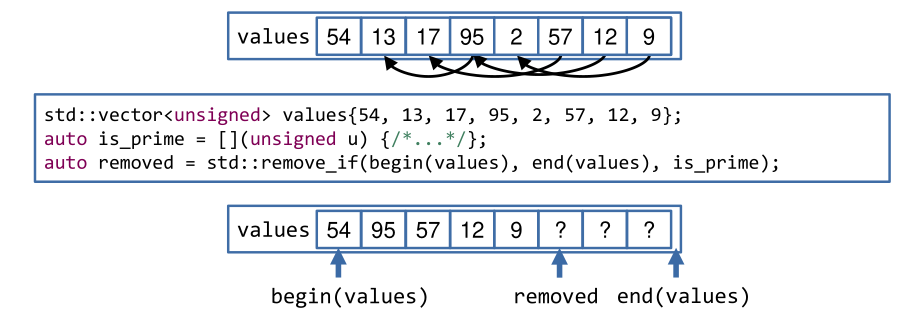
\includegraphics[width=.9\linewidth]{img/erase_remove_idiom.png}
\end{center}
\captionof{figure}{The Erase-Remove Idiom}
}


\textbf{Erase-Remove Idiom}
In data structures which are based on arrays, such as \texttt{std::vector}, removing every single element would be very time intensive.
To avoid this problem first all elements which should \textbf{not} be deleted are moved to the front.
After that only once the \texttt{erase} function is called and all deleted elements are erased / removed.

\textbf{Heap}

The STL itself has no heap data structure.
Instead, it uses a sequenced container to operate on.
The following functions always create a max heap, but the behavior could be changed using functors:
\begin{itemize}
\item \texttt{make\_heap()}: constructs a max heap
\item \texttt{pop\_heap()}: removes the largest element from a max heap
\item \texttt{push\_heap()}: adds an element to a max heap
\item \texttt{sort\_heap()}: turns a max heap into a range of elements sorted in ascending order
\end{itemize}

\textbf{for loops}

In \href{../../../roam/20210920103243-c.org}{CPP} exists three types of for loops:
\begin{itemize}
\item index based, do not used this, except you need the index
\item range base loops
\item iterator based loops
\end{itemize}


{
\begin{center}
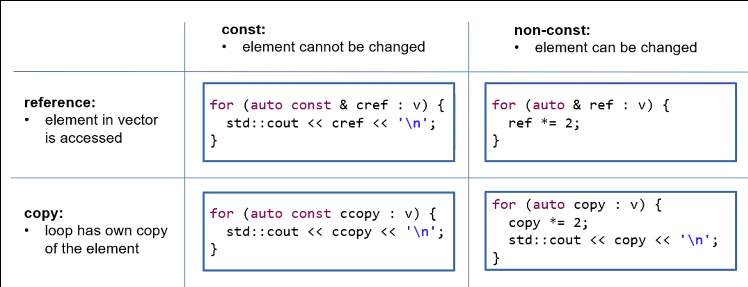
\includegraphics[width=.9\linewidth]{img/ranged_based_for_loop.png}
\end{center}
\captionof{figure}{Ranged-Based for loop}
}


This code is legacy and should not be used anymore.
Instead use the algorithms from the standard library.
\lstset{language=c++,label= ,caption= ,captionpos=b,numbers=none}
\begin{lstlisting}
for (auto it = std::begin(v); it != std::end(v); ++it) {
  std::cout << (*it)++ << ", ";
 }
\end{lstlisting}

\emph{Try to avoid programming your won loops (if possible)}: oftern algorithms faster, the correctness is proofed, and the readability of the code is better.


\textbf{lambdas}

Lambdas in \href{../../../roam/20210920103243-c.org}{CPP} have the following syntax:
\lstset{language=c++,label= ,caption= ,captionpos=b,numbers=none}
\begin{lstlisting}
[<capture>](<parameters>) -> <return-type> {
<statement>
  }
\end{lstlisting}

\lstset{language=c++,label= ,caption= ,captionpos=b,numbers=none}
\begin{lstlisting}
std::for_each(v.begin(), v.end(), [&out](auto x) {
  out << "print: " << x << '\n';
 });
\end{lstlisting}

Normally the return type does not have to be specified because the compiler can detect it correctly.
Lambdas are internally implemented as functors.

\section{Class}
\label{sec:org57de168}
\textbf{A good class}

A good class has:
\begin{itemize}
\item high cohesion
\item avoids deeply nested control structures
\item provides a guarantee about its state
\item properties for a value of the type that are always true \emph{(establish invariant)} if error during constructing throw exception
\end{itemize}


\textbf{classes and structs}

Normally you write the class declaration in the header file and the implementation is in the Header file.
The only difference between the keyword \texttt{class} and \texttt{strcut} is the default visibility.
\texttt{class} is per default private, \texttt{struct} public.
Additional to \texttt{public} and \texttt{private} there exits also the \texttt{protected} keyword. 

It is possible to declare your member variables as \texttt{const} but often this is the wrong way because this would prevent copy assignments.


\lstset{language=c++,label= ,caption= ,captionpos=b,numbers=none}
\begin{lstlisting}
/* Date.h */
struct Date {
  Date(int year);
  bool isLeapYear(int year);
  bool isValidDate() const;
};

/* Date.cpp */
Date::Date(int year)
  : year{year} {/**/}


bool Date::isLeapYear(int year) { /**/ }

bool Date::isValidDate() const { /**/ }
\end{lstlisting}

\textbf{Inheritance}

In \href{../../../roam/20210920103243-c.org}{CPP} multiple inheritance is possible.
To inherit from a class you write the following code:

\lstset{language=c++,label= ,caption= ,captionpos=b,numbers=none}
\begin{lstlisting}
class MyClass : public MyBase, private MyBase2 {
  int mvar;

public:
  MyClass(int i, int j) :
    MyBase{i}, MyBase2{}, mvar{j} {}
};
\end{lstlisting}

Normally the visibility is \texttt{public}.
But you can also set \texttt{protected} or \texttt{private}.
This specifies the maximum visibility of the elements inherit from the base class.

\textbf{Kinds of constructors}

In \href{../../../roam/20210920103243-c.org}{CPP} we have the following constructors which we can use in classes:
\begin{itemize}
\item default constructor
\item copy constructor
\item move constructor
\item type conversion constructor
\item list constructor
\end{itemize}


\textbf{How you should initialize member variables}
In the constructor you should do it like in the following snippet.
If you do it in an other way, the values are first default constructed and then reassigned.
\lstset{language=c++,label= ,caption= ,captionpos=b,numbers=none}
\begin{lstlisting}
Date(int year, int month, int day)
: year{year}, month{month}, day{day} {/**/}
\end{lstlisting}

If your class has some default values, you can initialize it directly in the header file.
This is called NSDMI (Non Static Data Member Initializers):
\lstset{language=c++,label= ,caption= ,captionpos=b,numbers=none}
\begin{lstlisting}
class Date {
  int year{9999}, month{12}, day{31};

  /**/
};
\end{lstlisting}

\textbf{Reimplement the default behaviour (constructor)}

Using the following syntax you can create the default constructor type again after creating a custom one.

\lstset{language=c++,label= ,caption= ,captionpos=b,numbers=none}
\begin{lstlisting}
class Date {
  Date(int year);
  Date() = default;
};
\end{lstlisting}

Using \texttt{delete} the implicit constructor type is removed

\lstset{language=c++,label= ,caption= ,captionpos=b,numbers=none}
\begin{lstlisting}
class Date {
  Date() = delete;
};
\end{lstlisting}

\textbf{Copy Constructor}

The copy constructor is a type of constructors in \href{../../../roam/20210920103243-c.org}{CPP} to copy all members to an new object.

\lstset{language=c++,label= ,caption= ,captionpos=b,numbers=none}
\begin{lstlisting}
struct Date {
  Date(Date const &)
};
\end{lstlisting}

\textbf{Move Constructor}

The move constructor is a type of constructors in \href{../../../roam/20210920103243-c.org}{CPP} to move all members to an new object.
\lstset{language=c++,label= ,caption= ,captionpos=b,numbers=none}
\begin{lstlisting}
struct Date {
  Date(Date const &&)
};
\end{lstlisting}

\textbf{Type Conversion Constructor}

The Type Conversion constructor is a type of constructors in \href{../../../roam/20210920103243-c.org}{CPP} to convert the input in the object.
It is recommended to set the \texttt{explicit} keyword.
If not set it could lead to unexpected conversions.

\lstset{language=c++,label= ,caption= ,captionpos=b,numbers=none}
\begin{lstlisting}
class Date {
  explicit Date(std::string const &);
};
\end{lstlisting}

\textbf{List Constructor}

The List Constructor is a type of constructors in \href{../../../roam/20210920103243-c.org}{CPP} to fill a container with content.

\lstset{language=c++,label= ,caption= ,captionpos=b,numbers=none}
\begin{lstlisting}
class Container {
  Container(std::initializer_list<Element> elements);
};

Container box{item1, item2, item3};
\end{lstlisting}

\textbf{Destructor}

The Destructor is the counter part to the constructor.
It must release all resources and is not allowed to throw an exception.
If you program properly you will hardly ever need to implement it yourself.
It is called automatically for local instances at the end of the block.

\lstset{language=c++,label= ,caption= ,captionpos=b,numbers=none}
\begin{lstlisting}
class Date {
  ~Date();
};
\end{lstlisting}

\textbf{Member Function}

It is a good practice to set as often as possible a member function as \texttt{const}.
This prevents you from changing \texttt{this}.
It is obvious that you can not call from a \texttt{const} member function a non-const member function.

\lstset{language=c++,label= ,caption= ,captionpos=b,numbers=none}
\begin{lstlisting}
/* Date.h */
class Date {
  bool isValidDate() const;
};


/* Date.cpp*/
bool Date::isValidDate() const { /**/ }
\end{lstlisting}

\textbf{Static Member Function}

Static Member Functions have some restrictions in \href{../../../roam/20210920103243-c.org}{CPP}.
In a static member function you can not access \texttt{this} (does not exits) and the function can not be \texttt{const} (again, \texttt{this} not exits).
The \texttt{static} keyword is only allowed in the declaration (header file).

\lstset{language=c++,label= ,caption= ,captionpos=b,numbers=none}
\begin{lstlisting}
/* Date.h */
struct Date {
  static isValidDate(int year);
};

/* Date.cpp */
Date::isValidDate(int year) { /**/ }
\end{lstlisting}

\textbf{Static Member Variable}

Similar to the static Member functions the \texttt{static} keyword occurs only in the header file.
If the variable is \texttt{const} the variable can be initialized directly in the header file.
If not it must be initialized in the \texttt{cpp} file.
But you should try to prevent non const static variables because they are a kind of global variables.

\lstset{language=c++,label= ,caption= ,captionpos=b,numbers=none}
\begin{lstlisting}
/* Date.h */
struct Date {
  static const int value{2};
  static int nonConst;
};

/* Date.cpp */
Date::nonConst = 4;
\end{lstlisting}

\textbf{Overriding Operators}

To override an operator in \href{../../../roam/20210920103243-c.org}{CPP} you use the following syntax:
\begin{itemize}
\item \texttt{<returnype> operator op(<parameters>);}
\end{itemize}
\lstset{language=c++,label= ,caption= ,captionpos=b,numbers=none}
\begin{lstlisting}
// free ooperator
Date operator+(Date const &rhs, Date const &lhs) { /* */ }


struct Date {
  /**/

  Date operator+(Date const &lhs) { /* */ }
};
\end{lstlisting}

\textbf{Non Overloadable Operators}

In \href{../../../roam/20210920103243-c.org}{CPP} the following operators are \textbf{not} overloadable:
\begin{itemize}
\item \texttt{::}
\item \texttt{.*}
\item \texttt{.}
\item \texttt{?}
\end{itemize}

\textbf{Free Operators}

Free Operators are operator overloads outside of the class definition.
\lstset{language=c++,label= ,caption= ,captionpos=b,numbers=none}
\begin{lstlisting}
Date operator+(Date const &rhs, Date const &lhs) { /* */ }
\end{lstlisting}

In this function it is \emph{not} possible to access the private / protected elements inside the class.

\textbf{Friend functions}

Functions with the keyword \texttt{friend} can only be declared inside a class declaration.
But the the function is \emph{not} part of the class itself.
It's a \emph{free} function which can also access the private member of a function.

This kind of function should only be used in exception cases.
For example for implementing the stream operators.

\lstset{language=c++,label= ,caption= ,captionpos=b,numbers=none}
\begin{lstlisting}
// Switch.h
class Switch {
  int state;

public:
  Switch();
  auto pressButton() -> void;

  friend auto operator<<(std::ostream &out, Switch sw) -> std::ostream&;
};

// Switch.cpp
Switch::Switch() : state{0} { }

auto Switch::pressButton() -> void {
  ++current;
  this->state = current % 3;
}

auto operator<<(std::ostream &out, Switch sw) -> std::ostream& {
  std::array<std::string, 3> arr = { "off", "on", "blinking" };
  out << arr[sw.state];
  return out;
}

\end{lstlisting}

\textbf{Member Operators}

Member Operators are operator overloads inside of the class definition.
\lstset{language=c++,label= ,caption= ,captionpos=b,numbers=none}
\begin{lstlisting}
struct Date {
  /**/

  Date operator+(Date const &lhs) { /* */ }
};
\end{lstlisting}

In this function it is possible to access the private / protected elements inside the class.


\textbf{Boost to implement compare operators}

Normally you have to implement all compare operators by your self.
Using the library Boost you only have to implement the less operator (\texttt{<}).
But in exchange you have to inherit from \texttt{boost::less\_than\_comparable<T>} (private is enough).

\lstset{language=c++,label= ,caption= ,captionpos=b,numbers=none}
\begin{lstlisting}
#include "boost/operators.hpp"
#include <tuple>


class Date : private boost::less_than_comparable<Date> {
  int year, month, day; 

public:
  bool operator<(Date const & rhs) const {
    return std::tie(year, month, day) < std::tie(rhs.year, rhs.month, rhs.day);
  }
}; 
\end{lstlisting}

\textbf{Overloading Stream Operators}

The syntax for use the output operator is the following:
\lstset{language=c++,label= ,caption= ,captionpos=b,numbers=none}
\begin{lstlisting}
std::cout << Date::myBirthday;
\end{lstlisting}

This requires that the \texttt{ostream} has an overload of the output operator with \texttt{Date} or the function is free.
We can not write an overload for \texttt{ostream} so only free operators are left.
But a free function can not access the private members of the class.
The solution to this problem are \texttt{friend} functions.
The same applies for the input operator and \texttt{istream}.


\lstset{language=c++,label= ,caption= ,captionpos=b,numbers=none}
\begin{lstlisting}
// Switch.h
class Switch {
  int state;

public:
  Switch();
  auto pressButton() -> void;

  // output
  friend auto operator<<(std::ostream &out, Switch sw) -> std::ostream&;
  friend auto operator>>(std::istream &in, Switch &sw) -> std::istream&;
};

// Switch.cpp
Switch::Switch() : state{0} { }

auto Switch::pressButton() -> void {
  ++current;
  this->state = current % 3;
}

auto operator<<(std::ostream &out, Switch sw) -> std::ostream& {
  std::array<std::string, 3> arr = { "off", "on", "blinking" };
  out << arr[sw.state];
  return out;
}

auto operator>>(std::istream &in, Switch &sw) -> std::istream& {
  std::array<State, 3> arr = { State::off, State::on, State::blinking };
  int i{0};
  in >> i;
  i = i % 3;

  if (in) {
    sw.state = arr[i];
  } else {
    throw std::invalid_argument{"Could not read a switch from input"};
  }
  return in;
}
\end{lstlisting}

\textbf{Factory Functions}

Place your factory function as a static member or in the same namespace.
The task of this function is to create the desired object and provide a default value.
This function are normally called:
\begin{itemize}
\item \texttt{make\_xxx()}
\item \texttt{create\_xxx()}
\end{itemize}

\lstset{language=c++,label= ,caption= ,captionpos=b,numbers=none}
\begin{lstlisting}
Date make_date(std::istream & in) {
  try {
    return Date{in};
  } catch(std::out_of_range const &) {
    return Date{9999, 12, 31};
  }
}
\end{lstlisting}

\section{Namespaces}
\label{sec:org80fa847}
\textbf{Namespaces}

Namespaces are used to group classes, functions and other elements and to prevent name clashes.
The same name can occur multiple times in different namespaces.
Namespaces can only defined outside classes and functions.
But the Namespace can be opened and closed multiple times.
Normally you open a namespace in the header file and reopen it in the cpp file again.

The global namespace in \href{../../../roam/20210920103243-c.org}{CPP} has the prefix \texttt{::} and can be ommited if unique.

\textbf{Import Namespace}

The keyword \texttt{using} is used to import a name from a namespace into the current scope.
Using type aliases you can shorten the name if its too long.
Using directives which import \textbf{ALL} names of a namespace should only be used locally (for example in a function).

\lstset{language=c++,label= ,caption= ,captionpos=b,numbers=none}
\begin{lstlisting}
#include <string>

auto foo() -> void {
  using namespace std;

  string a{"Hallo"};
}
\end{lstlisting}

\textbf{Anonymous Namespace}

Anonymous Namespaces are a special case of namespaces.
This namespaces are used to hide module internals like:
\begin{itemize}
\item helper function and types
\item constants
\end{itemize}


The anonymous namespace can not be imported by you.
The anonymous namespace is imported directly after the namespace is closed.
So the following elements can use the elements defined in the anonymous namespace.
You should anonymous namespaces only in the .cpp file.

\textbf{Argument Dependent Lookup / ADL}

When the compiler encounters an unqualified function or operator call with an argument of a user-defined type it tries to resolve it.
To resolve it checks the namespace of the arguments to find the function.

E.g it is not necessary to write \texttt{std::} in front of \texttt{for\_each} when \texttt{std::vector::begin()} is an argument.

\lstset{language=c++,label= ,caption= ,captionpos=b,numbers=none}
\begin{lstlisting}
// Date.h
namespace calendar {
  class Date {
    // ... 
  };

  bool isHoliday(Date const &);
}

// Holidays.cpp
#include "Date.h"

using Dates = std::vector<calendar::Date>;

void markHolidays(Dates const & dates) {
  for_each(begin(dates), end(dates), [](calendar::Date const & d) {
    if (isHoliday(d)) {} // this is found because of ADL
  });
}
\end{lstlisting}

\section{Enums}
\label{sec:orgeb75766}
\textbf{Enums}

In \href{../../../roam/20210920103243-c.org}{CPP} there exits two kinds of enums:
\begin{itemize}
\item unscoped enums
\item scoped enums
\end{itemize}


\lstset{language=c++,label= ,caption= ,captionpos=b,numbers=none}
\begin{lstlisting}
enum unscopedEnum {};
enum class scopedEnum {};
\end{lstlisting}

For enums the operators als can be overloaded
\lstset{language=c++,label= ,caption= ,captionpos=b,numbers=none}
\begin{lstlisting}
DayOfWeek operator++(DayOfWeek &); // prefix
DayOfWeek operator++(DayOfWeek &, int); // postfix
\end{lstlisting}

The enumerator names are not mapped automatically to their name.
You have to provide a lookup table to print out the name.

\lstset{language=c++,label= ,caption= ,captionpos=b,numbers=none}
\begin{lstlisting}
std::ostream & operator<<(std::ostream & out, Month m) {
  static std::array<std::string, 12> const monthNames {
    "Jan", "Feb", "Mar", "Apr", "May", "Jun",
    "Jul", "Aug", "Sep", "Oct", "Nov", "Dec" };
  out << monthNames[m - 1]; //m - 1 if Jan has value 1
  return out;
}
\end{lstlisting}

\textbf{Scoped / Unscoped}

Unscoped enums can be converted to \texttt{int} implicit.
Scoped enums can only explicitly casted.
For the conversation from \texttt{int} to enum is always the \texttt{static\_cast} required.

\lstset{language=c++,label= ,caption= ,captionpos=b,numbers=none}
\begin{lstlisting}
enum DayOfWeek { Sun, /* ... */ };
enum class Month { Jan, /* ... */ };

int day = Sun;
int month = static_cast<int>(Month::Jan);
\end{lstlisting}

Unscoped enums are best used as a memeber of a class.
If the enum is a independent type then the scoped version should be used.

\textbf{Specifying the Underlying type for an enum}

In CPP you can specify which size the elements of the enum should have.
\emph{Attention}: This is \emph{not} a inheritance, you only specify the underlying type.
\lstset{language=c++,label= ,caption= ,captionpos=b,numbers=none}
\begin{lstlisting}
enum class LaunchPolicy : unsinged char { /**/ };
\end{lstlisting}

\section{Templates}
\label{sec:org7890c3c}
\subsection{Function Templates}
\label{sec:org1fd4d06}
\textbf{inline keyword}
\begin{quote}
Because the meaning of the keyword inline
for functions came to mean
"multiple definitions are permitted"
rather than "inlining is preferred",
that meaning was extended to variables. 
\end{quote}

\textbf{What are Function Templates}

If you want to implement the \texttt{min} method have to implement this for \texttt{int}, \texttt{float}, \texttt{double} and so on.
This is error prone because you would write the same code for each data type you want to support.
In \href{../../../roam/20210920103254-programming_language.org}{Programming Language}s like \href{../../../roam/20211003114158-c.org}{C\#} or \href{../../../roam/20201116150053-java.org}{Java} you have Generics to solve this problem.
In \href{../../../roam/20210920103243-c.org}{CPP} we have Function Templates for compile-time polymorphism.

These are normally defined in a header file because the compiler needs to see the whole template to create an instance.

\lstset{language=c++,label= ,caption= ,captionpos=b,numbers=none}
\begin{lstlisting}
template <typename T>
T min(T left, T right) {
  return left < right ? left : right;
}
\end{lstlisting}

\textbf{How do Function Templates work}

The process how the compiler generates code from a Function Template.

The compiler\ldots{}:
\begin{enumerate}
\item resolves the function template
\item figures out the template arguments
\item creates code with template parameters replaced
\item checks the types for correct usage
\end{enumerate}


{
\begin{figure}[htbp]
\centering
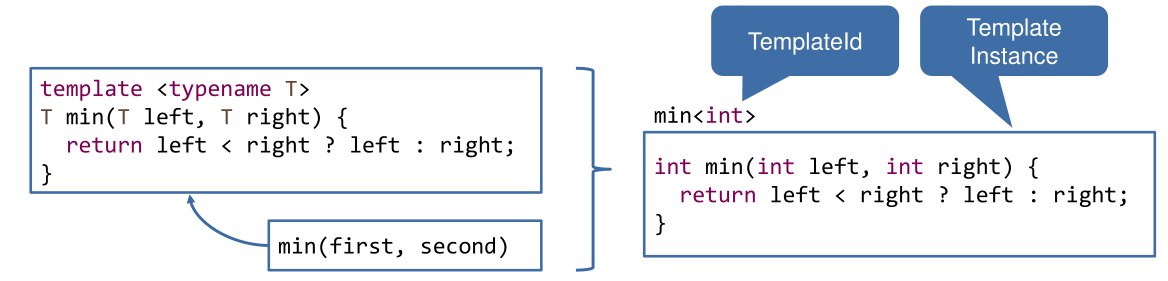
\includegraphics[width=.9\linewidth]{img/template_instantiation.png}
\caption{Example instantiation with the min function}
\end{figure}
}

\textbf{Type Checking in Templates}

The type checking in templates happens twice:
\begin{enumerate}
\item when the template is defined: Only basic checks are performed (syntax, name resolution)
\item when the template is instantiated (used): the compiler checks whether the template arguments can be used as required by the template
\end{enumerate}


\textbf{Valid Template Argument}

\href{../../../roam/20210920103243-c.org}{CPP} use duck-typing to check if template argument is valid for this template.
If the code inside the function can be executed using the given type then the template is valid.
Otherwise, a compilation error is thrown.

\emph{Example}: 

What are the requirements of the type T in the \texttt{min} function template?
\lstset{language=c++,label= ,caption= ,captionpos=b,numbers=none}
\begin{lstlisting}
template <typename T>
T min(T left, T right) {
  return left < right ? left : right;
}
\end{lstlisting}

\begin{itemize}
\item T must be comparable with the \texttt{<} operator
\item Copy / Move construcible, to return T by value
\end{itemize}


\textbf{duck-typing}

Duck-typing is concept where the type of variable is not describe using its class but using the existence of methods, properties, fields.

\begin{quote}
When I see a bird that walks like a duck and swims like a duck and quacks like a duck, I call that bird a duck.
\end{quote}

\textbf{Template Argument Deduction}

The process of figuring out the correct template arguments from the call.
The \href{../../../roam/20210920103243-c.org}{CPP} compiler performs a pattern matching on the function parameter list for deducing the correct argument.

If ambiguities during the deduction occurs then a compiler error is throws.


{
\begin{figure}[htbp]
\centering
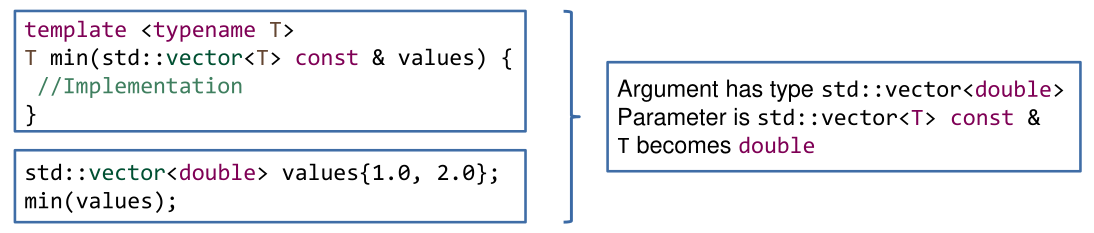
\includegraphics[width=.9\linewidth]{img/template_argument_deduction.png}
\caption{Example of Template Argument Deduction}
\end{figure}
}

\textbf{Function Template Overloading}

Using string literals in a normal template could be lead to wrong behavior.
The \texttt{min} template below (\ref{fig:missingTemplate}) is implemented correctly.
But if you use it with string literals a comparison of the address is made.
This is normally not what you want.

{
\begin{center}
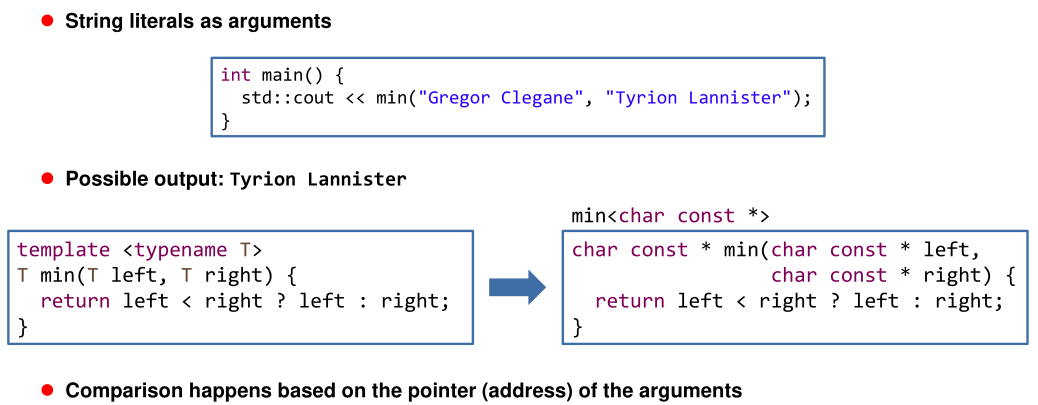
\includegraphics[width=.9\linewidth]{img/missing_template_overloadin.png}
\end{center}
\captionof{figure}{Missing Template Overloading}\label{fig:missingTemplate}
}


To prevent this behavior you could overwrite a template.
Multiple function template with the same name can exist as long as they can be distinguished by their parameter list.
It is also possible to write a \emph{normal} function with the same name.
The most concrete version is used in this case.

\lstset{language=c++,label= ,caption= ,captionpos=b,numbers=none}
\begin{lstlisting}
template <typename T>
T min(T left, T right) {
  return left < right ? left : right;
}

template <typename T>
T * min(T * left, T * right) {
  return *left < *right ? left : right;
}

char const * min(char const * left,
		 char const * right) {
  return std::string{left} < std::string{right} ? left : right;
}
\end{lstlisting}

\subsubsection{Variadic Templates}
\label{sec:orge99275a}
\textbf{Variadic Templates}

In some cases the number of template parameters might not be fixed / known before.
Thus, the template shall take an arbitrary number of parameters.

\lstset{language=c++,label= ,caption= ,captionpos=b,numbers=none}
\begin{lstlisting}
template<typename First, typename...Types>
void printAll(First const & first, Types const &...rest) {
  std::cout << first;
  if (sizeof...(Types)) {
    std::cout << ", ";
  }
  printAll(rest...);
}
\end{lstlisting}

\textbf{Pack Expansion}

In a Variadic Template the last parameter is a function is called Function Parameter Pack.
In the template declaration it is called Template Parameter Pack.
This pack contains all remaining parameters.

Using \texttt{sizeof...(PackType)} the number of elements in the template parameter pack is returned.

To expand if \texttt{rest...} syntax is used.
This expands to a comma seperated list of instances of the pattern (see example).

The pattern must contain at least one pack parameter.
The base case for the recursion must exist \textbf{before} the templates is executed / generated.
Otherwise an compilation error is thrown.



{
\begin{center}
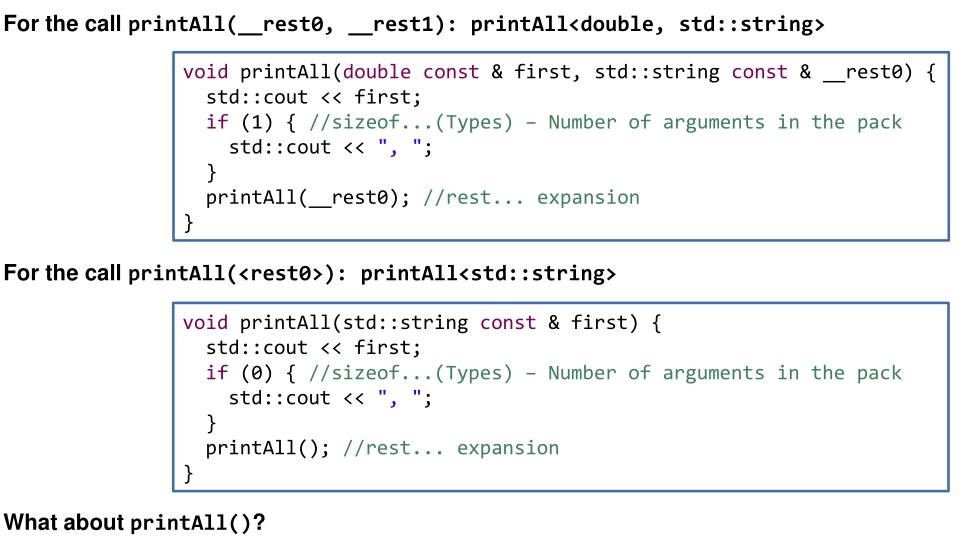
\includegraphics[width=.9\linewidth]{img/variadic_template_pack_expansion.png}
\end{center}
\captionof{figure}{Compiler output from pack expansion}
}

\subsection{Class Templates}
\label{sec:org2d9e1a4}
\textbf{Class Template}

Class Templates are very similar to function templates.
Instead of function it is based on classes.
Therefore, it enables us compile-time polymorphism for classes and structs.

\lstset{language=c++,label= ,caption= ,captionpos=b,numbers=none}
\begin{lstlisting}
template <typename T>
class Sack {
  using SackType = std::vector<T>;
  using size_type = typename SackType::size_type;
  SackType theSack{};
public:
  bool empty() const {
    return theSack.empty();
  }
  size_type size() const {
    return theSack.size();
  }
  void putInto(T const & item) {
    theSack.push_back(item);
  }
  T getOut(); // implementation somewhere else
};


// example for implementing member functions outside of a class
template <typename T>
inline T Sack<T>::getOut() {
  if (empty()) {
    throw std::logic_error{"Empty Sack"};
  }
  auto index = static_cast<size_type>(rand() % size());
  T retval{theSack.at(index)};
  theSack.erase(theSack.begin() + index);
  return retval;
}
\end{lstlisting}


\textbf{Access to a type of the template parameter}

Within a template definition sometimes you want to use names witch are directly or indirectly depending on the template parameter.
In the example below for example the \texttt{size\_type} from \texttt{SackType}.
In contrast to a variable or function name you have to tell the compiler that it is a type.
This is done using the \texttt{typename} keyword.

In the example below the \texttt{size\_type} of Sack and the \texttt{size\_type} of \texttt{SackType} / \texttt{std::vector} are the same.

\lstset{language=c++,label= ,caption= ,captionpos=b,numbers=none}
\begin{lstlisting}
template <typename T>
class Sack {
  using SackType = std::vector<T>;
  using size_type = typename SackType::size_type;
  SackType theSack{};
}
\end{lstlisting}


{
\begin{center}
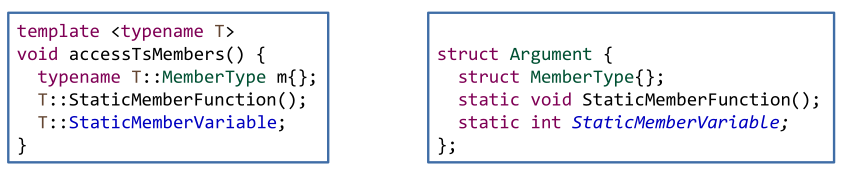
\includegraphics[width=.9\linewidth]{img/accessing_member_of_template_parameter.png}
\end{center}
\captionof{figure}{Accessing a member of a template parameter}
}

\textbf{static member variables in class templates}

In a class template you can create a static variable.
This does not violate the ODR.
Since C++17 it is possible to declare the static variable inside the class template.
However, this requires the \texttt{inline} keyword.


\lstset{language=c++,label= ,caption= ,captionpos=b,numbers=none}
\begin{lstlisting}
template <typename T>
struct staticmember {
  inline static int dummy{sizeof(T)};
};
\end{lstlisting}

\textbf{Class Template Gotchas}

When a class template inherits from another class template the name-lookup can be surprising!
To prevent this behavior always use \texttt{this->} or \texttt{name::} to refer to an inherited member.

{
\begin{center}
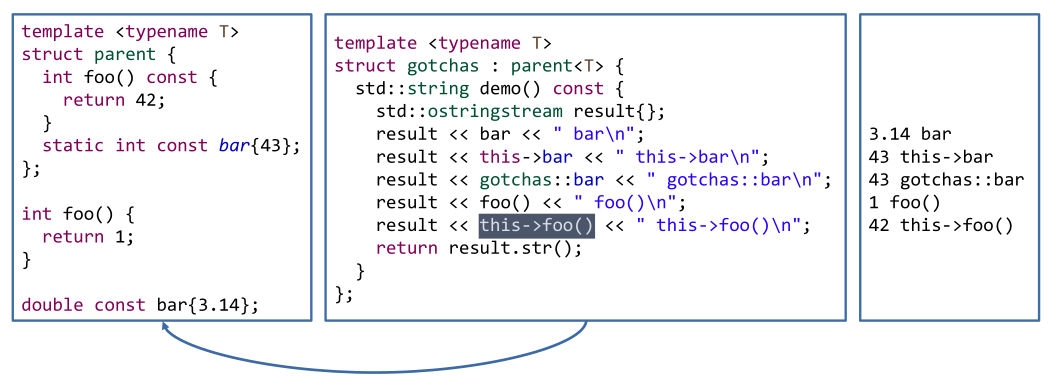
\includegraphics[width=.9\linewidth]{img/class_template_gotchas.png}
\end{center}
\captionof{figure}{Class Template Gotchas Example}
}

\textbf{Class Template Specialization}

Similar to the overloads in a function template you could specialize a class template.
Thus, we provide different implementations based on the template parameter.
It is possible to provide a partial specialization or an explicit specialization (a specialization for a concrete type).

{
\begin{center}
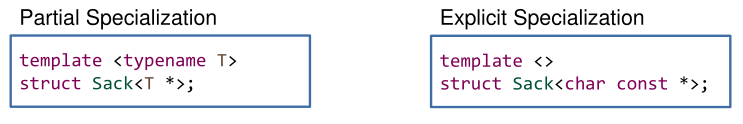
\includegraphics[width=.9\linewidth]{img/partial_explicit_specialization.png}
\end{center}
\captionof{figure}{Partial and Explicit Specialization}
}

\textbf{How to prevent the compiler from creating specialiced class template}

In our Sack example using class templates we do not want raw pointers (this could lead to dangling pointers).
To prevent the compiler to create such an instance we could write the following code:

\lstset{language=c++,label= ,caption= ,captionpos=b,numbers=none}
\begin{lstlisting}
template <typename T>
struct Sack<T> {
  /* implementation */
};

/* */
template <typename T>
struct Sack<T *> {
  ~Sack() = delete;
};
\end{lstlisting}

Because the destructor is missing the compiler could not create such an instance (except you use \texttt{new} - DO NOT DO THIS).

\textbf{How to inherit constructors in a class template}

If you want to implement a class template which inherits from an other class template you may want to inherit its constructors.
This is also done using the \texttt{using} keyword:

\lstset{language=c++,label= ,caption= ,captionpos=b,numbers=none}
\begin{lstlisting}
template<typename T>
struct safeVector : std::vector<T> {
  using container = std::vector<T>;
  using container::container; //or using std::vector<T>::vector; Inherit constructors
  using size_type = typename container::size_type;
  using reference = typename container::reference;
  using const_reference = typename container::const_reference;
  reference operator[](size_type index) {
    return this->at(index);
  }
  const_reference operator[](size_type index) const {
    return this->at(index);
  }
  // should also provide front/back with empty() check
};
\end{lstlisting}

\textbf{Deduction Guides}

Deduction Guides are used to tell the compiler how to translate a set of constructor arguments into template parameters for the class.

In the following code snippet I have to tell the compiler how to map the Template Parameter \texttt{Iter}.
Otherwise, the compiler would not know that \texttt{Iter} should be an iterator.
It could be also an \texttt{int} or anything else.


\lstset{language=c++,label= ,caption= ,captionpos=b,numbers=none}
\begin{lstlisting}
template <typename T>
class Sack {
  //...
  template <typename Iter>
  Sack(Iter begin, Iter end) : theSack(begin, end) {}
  //...
};

// deduction guide
template <typename Iter>
Sack(Iter begin, Iter end) -> Sack<typename std::iterator_traits<Iter>::value_type>;
\end{lstlisting}


\textbf{template template parameters}

A template can take templates as parameters.
This parameter is called template template parameter.

\lstset{language=c++,label= ,caption= ,captionpos=b,numbers=none}
\begin{lstlisting}
// variadic template is required because many stl containers needs more than one element type
template<typename T, template<typename...> typename Container>
class Sack;

Sack<unsigned, std::set> aSack{1, 2, 3}; 
\end{lstlisting}

\textbf{Default for a template parameter}

Sometimes you want to sepcify a default for a template parameter.
This is done like in the following snippet.

\lstset{language=c++,label= ,caption= ,captionpos=b,numbers=none}
\begin{lstlisting}
template <typename T, template<typename...> typename Container = std::vector>
class Sack;
\end{lstlisting}

\textbf{non-type template parameters}

In some cases you want not a type but a value as a parameter in the template.
For example the \texttt{std::array} has one type and one non-type parameter.
The second one is the size of the array.

If you want a flexible type you can also use \texttt{auto}.

\lstset{language=c++,label= ,caption= ,captionpos=b,numbers=none}
\begin{lstlisting}
template <typename T, std::size_t n>
auto average(std::array<T, n> const & values) {
  auto sumOfValues = accumulate(begin(values), end(values), 0);
  return sumOfValues / n;
}
\end{lstlisting}

\section{Heap Memory Management}
\label{sec:orgf7c6916}

\textbf{RAII - Resource Acquisition Is Initialization}

Resource Acquisition Is Initialization (RAII) is a concept used in programming.
The concept says:
\begin{itemize}
\item allocation of resources should happen in the constructor
\item deallocation should happen in the destructor
\end{itemize}


The benefit of this pattern is that in every case the resources are allocated correctly and deallocated.


\lstset{language=c++,label= ,caption= ,captionpos=b,numbers=none}
\begin{lstlisting}
struct RaiiWrapper {
  RaiiWrapper() {
    //Allocate Resource
  }
  ~RaiWrapper() {
    //Deallocate Resource
  }
};
\end{lstlisting}

\textbf{How you should manage heap memory}

In modern \href{../../../roam/20210920103243-c.org}{CPP} you should never allocate memory directly on the heap (\texttt{new} keyword).
Instead, you should use libraries for this (where possible).
Those libraries normally implement the \href{../../../roam/20220118172628-resource_acquisition_is_initialization.org}{Resource Acquisition Is Initialization} idiom.

The CPP STL provides a few types for heap management (smart pointers).

\textbf{Smart Pointers}

\begin{itemize}
\item std::unique\textsubscript{ptr}<T> obtained with std::make\textsubscript{unique}<T>()
\item std::shared\textsubscript{ptr}<T> obtained with std::shared<T>()
\end{itemize}


\textbf{unique\textsubscript{ptr}}

The unique\textsubscript{ptr} is a smart pointer used for unshared memory.
Only a single owner exists.
It is often used to wrap to-be-freed pointers from C functions when interfacing legacy code.
\texttt{std::unique\_ptr} can not be used for class hierarchies.


\lstset{language=c++,label= ,caption= ,captionpos=b,numbers=none}
\begin{lstlisting}
#include <iostream>
#include <memory>
#include <utility>

std::unique_ptr<int> create(int i) {
  return std::make_unique<int>(i);
}

int main() {
  std::cout << std::boolalpha;
  auto pi = create(42);
  std::cout << "*pi = " << *pi << '\n';
  std::cout << "pi.valid? " << static_cast<bool>(pi) << '\n';
  auto pj = std::move(pi);
  std::cout << "*pj = " << *pj << '\n';
  std::cout << "pi.valid? " << static_cast<bool>(pi) << '\n';
}
\end{lstlisting}

\textbf{shared\textsubscript{ptr}}

The shared\textsubscript{ptr} is a smart pointer.
The shared\textsubscript{ptr} works similar to \href{../../../roam/20201116150053-java.org}{Java}s references.
It can be copied and passed around.
The last one ceasing to exist deletes the object.
You can create a \texttt{std::shared\_ptr} using \texttt{std::make\_shared<T>()}

\emph{Attention}: All owners of the shared\textsubscript{ptr} can changed the value of it.


\lstset{language=c++,label= ,caption= ,captionpos=b,numbers=none}
\begin{lstlisting}
struct Article {
  Article(std::string title, std::string content);
  //..
};
Article cppExam{"How to pass CPl?", "In order to pass the C++ exam, you have to..."};
std::shared_ptr<Article> abcPtr = std::make_shared<Article>("Alphabet", "ABCDEFGHIJKLMNOPQRSTUVXYZ");
\end{lstlisting}


The shared\textsubscript{ptr} is used when you want to create your own object networks.
Another situation is when you need run-time polymorphic or class members that can not be passed as reference, e.g., because of lifetime issues.

\textbf{weak\textsubscript{ptr}}

The weak\textsubscript{ptr} is similar to the shared\textsubscript{ptr}.
But a weak\textsubscript{ptr} does not increment the counter of the shared\textsubscript{ptr}.
Therefore, using weak\textsubscript{ptr} you can break cyclic dependencies.

The function \texttt{std::weak\_ptr::lock()} returns a \texttt{std::shared\_ptr} that either points to the alive pointer or is empty.


\lstset{language=c++,label= ,caption= ,captionpos=b,numbers=none}
\begin{lstlisting}
struct Person {
  std::shared_ptr<Person> child;
  std::weak_ptr<Person> parent;
  void Person::acquireMoney() const {
    auto locked = parent.lock();
    if (locked) {
      begForMoney(*locked);
    } else {
      goToTheBank();
    }
  }
};
\end{lstlisting}

\textbf{weak\textsubscript{ptr} from this}

It would be nice if parents could spawn their own children.
Therefore, we need a \texttt{std::weak\_ptr} to the \texttt{this} object which is assigned to \texttt{child.parent}.
This could be done by inheriting from \texttt{std::enable\_shared\_from\_this<T>}.

{
\begin{center}
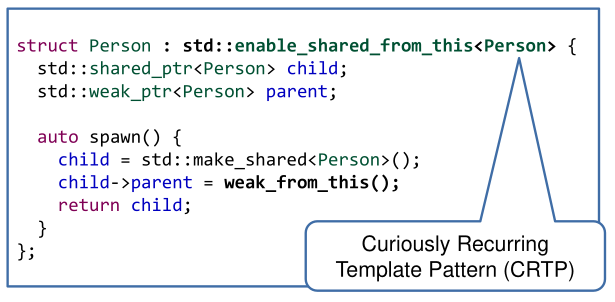
\includegraphics[width=.9\linewidth]{img/enable_shared_from_this.png}
\end{center}
\captionof{figure}{Create weak_ptr from this}
}

\section{Dynamic Polymorphism}
\label{sec:org271b08f}
\textbf{mix-in}

Mix-in is something like a class which provide additional functionality without adding more data.
In \href{../../../roam/20210920103243-c.org}{CPP} these arte often classes which requires your own class as template argument.

\lstset{language=c++,label= ,caption= ,captionpos=b,numbers=none}
\begin{lstlisting}
struct Date : boost::equality_comparable<Date> {
  //...
};
\end{lstlisting}

\textbf{shadowing member functions}

If you reimplemented a function in a derived class it shadows its counterpart in the base class.
Even if the signature does not match (constness is part of the signature).
However, if access through a declared base object, the shadowing is ignored and only the base class members are availabel (static dispatch).
The static dispatch is the default in CPP.

If you want in your subclass both members (from sub and base class) you need to \emph{import} using the keyword \texttt{using} (see figure \ref{fig:resoulutionShadowing}).

The output of in figure \ref{fig:shadowing} below is \emph{Hi, I'm Base}.


{
\begin{center}
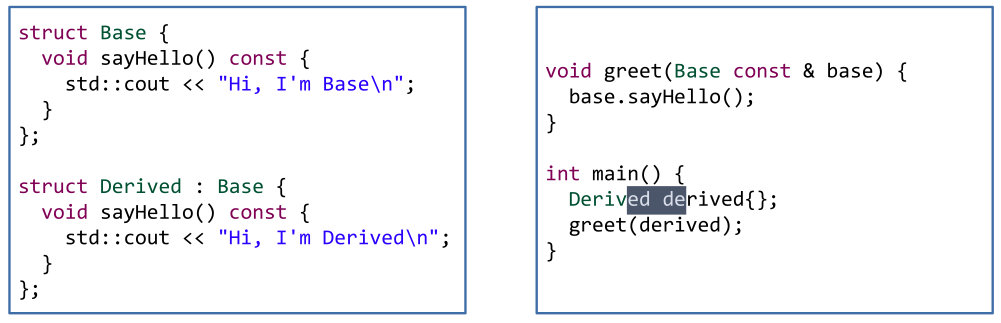
\includegraphics[width=.9\linewidth]{img/shadowing_member_functions.png}
\end{center}
\captionof{figure}{Shadowed Member Function}\label{fig:shadowing}
}


{
\begin{center}
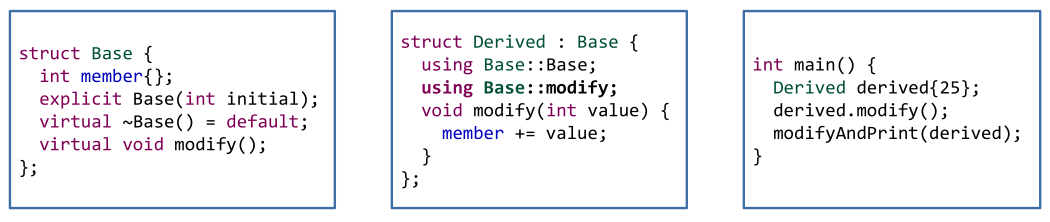
\includegraphics[width=.9\linewidth]{img/shadowing_member_functions_using.png}
\end{center}
\captionof{figure}{Resolution for Hidden Member}\label{fig:resolutionShadowing}
}

\textbf{virtual member functions}

To use dynamic polymorphism the function requires keyword \texttt{virtual}.
The \texttt{virtual} keyword can be omitted in the derived class.
Similar to \href{../../../roam/20201116150053-java.org}{Java}s annotation \texttt{@Override} you can add the \texttt{override} keyword to the function.

For a successful override the function signature must be the same (also the constness).

{
\begin{center}
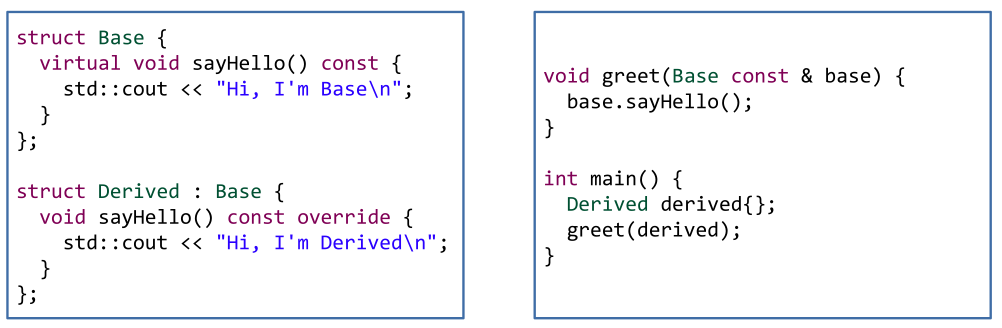
\includegraphics[width=.9\linewidth]{img/virtual_member_function.png}
\end{center}
\captionof{figure}{Virtual Member Function}
}

\textbf{Call Virtual Member Functions}

In \href{../../../roam/20210920103243-c.org}{CPP} if you want dynamic polymorphism you need a reference or pointers.
If you only have a value object of the base class also the base function is called.


\#+LATEX \{
\begin{center}
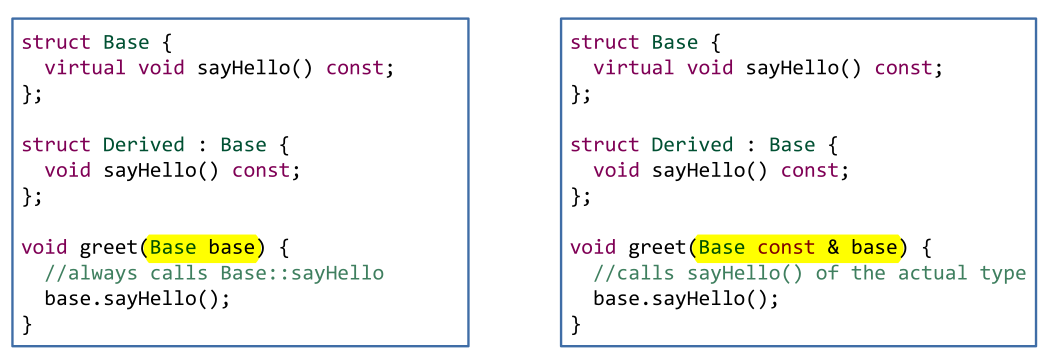
\includegraphics[width=.9\linewidth]{img/calling_virtual_member_functions.png}
\end{center}
\captionof{figure}{Example how to call virtual member functions}
\#+LATEX \}

\#+LATEX \{
\begin{center}
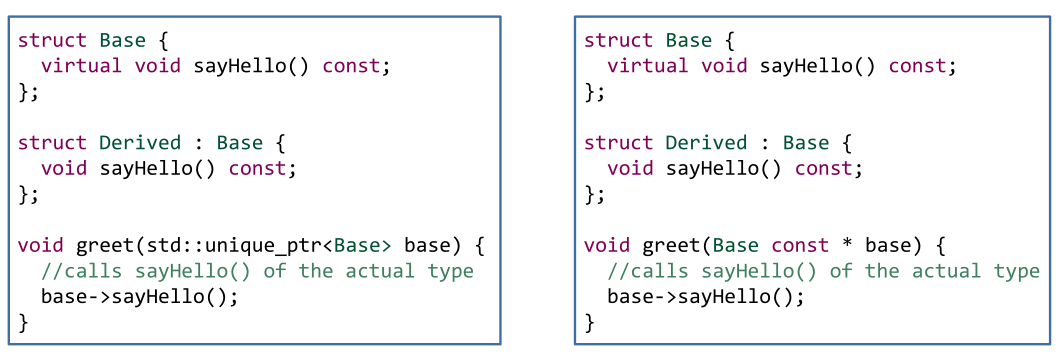
\includegraphics[width=.9\linewidth]{img/virtual_member_function2.png}
\end{center}
\captionof{figure}{Example 2 how to call virtual member functions}
\#+LATEX \}

\textbf{Pure Virtual Function}

In \href{../../../roam/20210920103243-c.org}{CPP} does not exist interfaces.
Using pure virtual functions you make a class abstract.
This can sometimes behave similar to an interface.


\lstset{language=c++,label= ,caption= ,captionpos=b,numbers=none}
\begin{lstlisting}
struct AbstractBase {
  virtual void doitnow() = 0;
};
\end{lstlisting}

\textbf{Virtual Member Functions using smart pointers}

If you have virtual members in your class then you need a virtual destructor if it is you used with a unique\textsubscript{ptr}.
Otherwise, only the destructor of the base is called.

The shared\textsubscript{ptr} memorize the actual type and know which destructor to call.
Thus, the destructor is not required to be virtual.

\textbf{Object Slicing}

When in \href{../../../roam/20210920103243-c.org}{CPP} a function takes a base class as value parameter, but you provide a subclass then \emph{object slicing} occurs.
That means, that the base is extracted / sliced from the subclass and passed to the function.
Therefore, functions which were overwritten are not available (see figure \ref{fig:slicing}).

Somthing similar happens if you assign a subclass to a base class reference.
The creation of the reference is OK.
But the second assignment copies only the base class part into the base reference (see figure \ref{fig:refsclicing}).
To prevent this, you can declare the copy-operations as deleted

\lstset{language=c++,label= ,caption= ,captionpos=b,numbers=none}
\begin{lstlisting}
struct Book {
  //...
  Book & operator=(Book const & other) = delete;
  Book(Book const & other) = delete;
};

// does not compile anymore because copy-operations are deleted
EBook designPatterns{writeEbook(395)};
EBook refactoring{writeEbook(430)};
refactoring.openPage(400);
Book & some = refactoring;
some = designPatterns;
readPage(some.currentPage());
\end{lstlisting}


{
\begin{center}
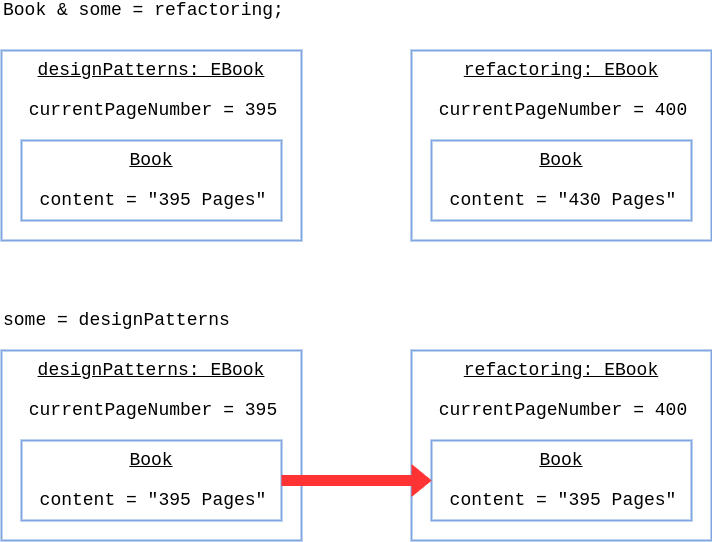
\includegraphics[width=.9\linewidth]{img/object_slicing_in_references.png}
\end{center}
\captionof{figure}{Slicing in references}\label{fig:refslicing}
}


{
\begin{center}
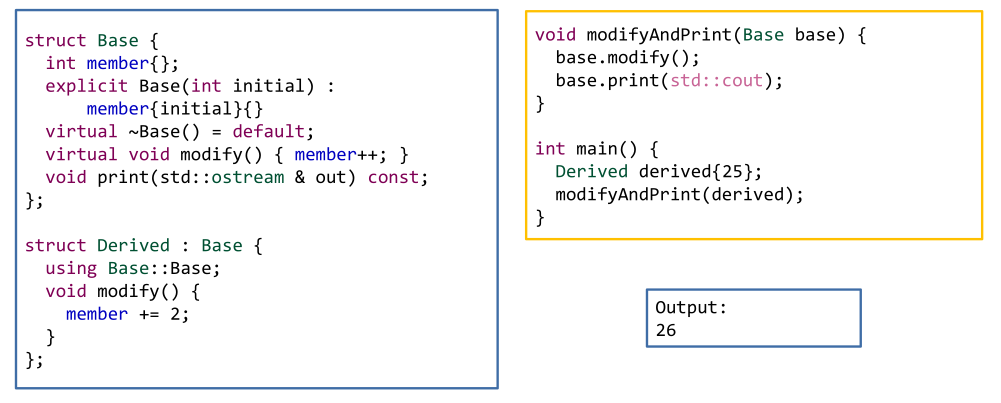
\includegraphics[width=.9\linewidth]{img/object_slicing.png}
\end{center}
\captionof{figure}{Example of object slicing}\label{fig:slicing}
}


\textbf{Guidelines}

\begin{itemize}
\item You should only apply inheritance and virtual member functions if you know what you do
\item Do not (like the IDE) create classes with virtual members by default
\item mark overwritten functions in sub classes with override
\item If you design base classes with polymorphic behavior, understand the common abstraction that they represent
\begin{itemize}
\item Extract from existing class(es) the base after you see the commonality arise
\end{itemize}
\item Follow the Liskov Substitution Principle
\item Do not break invariants of the base class
\item Beware of unwanted member hiding
\item Avoid object slicing
\item Mark Destructors virtual if you have any other virtual member function
\end{itemize}

\section{Initialization and Aggregates}
\label{sec:org1ca3f05}
\textbf{Kinds of initialization}

\href{../../../roam/20210920103243-c.org}{CPP} has many of initialization.
\begin{itemize}
\item Default Initialization
\item Value Initialization
\item Direct Initialization
\item Copy Initialization
\item List Initialization
\item Aggregate Initialization
\end{itemize}


Which kind is used is based on the context.

\textbf{Default Initialization}

The Default Initialization is the simplest one in \href{../../../roam/20210920103243-c.org}{CPP}.
You simply don't provide an initializer.
The result depends on the kinds of entity we declare.
Default Initialization could be dangerous because it sometimes behaves unexpected.

\lstset{language=c++,label= ,caption= ,captionpos=b,numbers=none}
\begin{lstlisting}
int global_variable; // implicitly static
void di_function() {
  static long local_static;
  long local_variable;
}
struct di_class {
  di_class() = default;
  char member_variable; // not in ctor init list
};
\end{lstlisting}

Static variables are zero initialized first and then their default constructor is called.
If the type can not be default constructed the program does not compile.
Non-static integral and floating point variables are uninitialized.
Objects of class types are constructed using their default constructor.
Member variables not in a ctor-init-list are default initialized.

\textbf{Value Initialization}

The Value Initialization is performed with empty \texttt{()} or \texttt{\{\}}.
However, you should use the \texttt{\{\}} since it works in more cases (see example below).
The Value Initialization just calls the default constructor for class types.

\lstset{language=c++,label= ,caption= ,captionpos=b,numbers=none}
\begin{lstlisting}
#include <string>
#include <vector>
void vi_function() {
  int number { };
  std::vector<int> data { };
  std::string actually_a_function(); // you define here a new function!!!
}
\end{lstlisting}

\textbf{Direct Initialization}

The Direct Initialization is one type of initialization in CPP.
The Direct Initialization works similar to the value initialization.
It uses non-empty \texttt{()} or \texttt{\{\}}.
When you use \texttt{\{\}} this only applies if you want to initialize not a class type.
Still you should prefer the \texttt{\{\}} syntax.

In the example below the last line is a function declaration of a function returning a word and taking an unnamed pointer to a function returning a string.

\lstset{language=c++,label= ,caption= ,captionpos=b,numbers=none}
\begin{lstlisting}
#include <string>
void diri_function() {
  int number{32};
  std::string text("CPl");
  word vexing (std::string()); 
}
\end{lstlisting}

\textbf{Copy Initialization}

To invoke the copy initialization the \texttt{=} is used.

\begin{itemize}
\item If the object has class type and the right-hand side has the same type:
\begin{itemize}
\item if the right-hand side is temporary, the object is constructed "in-place"
\item otherwise, the copy constructor is invoked
\end{itemize}
\item Otherwise, a suitable conversion is searched for.
\end{itemize}

This applies also to return / throw / catch statements.

\lstset{language=c++,label= ,caption= ,captionpos=b,numbers=none}
\begin{lstlisting}
#include <string>
std::string string_factory() { return ""; }
void ci_function() {
  std::string in_place = string_factory();
  std::string copy = in_place;
  std::string converted = "CPl";
}
\end{lstlisting}

\textbf{List Initialization}

The list initialization uses the non-empty \texttt{\{\}}.
Further there exists two kinds of the list initialization:
\begin{itemize}
\item direct list initialization
\item copy list initialization
\end{itemize}


The constructor is selected in two phases:
\begin{enumerate}
\item if there is a suitable constructor taking \texttt{std::initializer\_list}, it is selected
\item otherwise, a suitable constructor is searched., it is selected
\end{enumerate}


\emph{Attention}: Since \texttt{std::initializer\_list} is preferred, you might run into trouble.


\lstset{language=c++,label= ,caption= ,captionpos=b,numbers=none}
\begin{lstlisting}
std::string direct { "CPl" };
std::string copy = { "CPlA" };
std::vector<int> data {10, 42}; // creates [10, 42] and not 42x 10
std::vecotr<int> data2(10, 42); // create 42x 10
return data[5]; // Undefined Behaviour
\end{lstlisting}

\textbf{Aggregate Initialization}

The Aggregate Initialization is a special case of the list initialization.
If the type is an aggregate then the members and base classes are initialized from the list.
If you provide fewer initializers than there are bases and members the \emph{uninitialized} members used the list from the declaration or the empty list.

\lstset{language=c++,label= ,caption= ,captionpos=b,numbers=none}
\begin{lstlisting}
struct person {
  std::string name;
  int age{42};
  bool operator<(person const & other) const {
    return age < other.age;
  }
  void write(std::ostream & out) const {
    out << name << ": " << age << '\n';
  }
};

int main() {
  person rudolf{"Rudolf", 32};
  rudolf.write(std::cout); // Rudolf: 32

  person hans{"Hans"};
  hans.write(std::cout); // Hans: 42
}
\end{lstlisting}

\textbf{Aggregates in CPP}

Aggregates are simple class types which are often used for DTOs.
They can have other types as public base classes.
They can provide member variables and functions.
But they don't have a user-provide, inherited or explicit constructors.
They also don't have any protected or private direct fields.


\lstset{language=c++,label= ,caption= ,captionpos=b,numbers=none}
\begin{lstlisting}
struct person {
  std::string name;
  int age{42};
  bool operator<(person const & other) const {
    return age < other.age;
  }
  void write(std::ostream & out) const {
    out << name << ": " << age << '\n';
  }
};
int main() {
  person rudolf{"Rudolf", 32};
  rudolf.write(std::cout);
}
\end{lstlisting}

\textbf{What is a DTO}

DTO is short for Data Transfer Object.
That is a class which is only used to group information to transfer it from one point to another.
Therefore, they normally don't have any invariant.
\section{CUTE}
\label{sec:org7d96e27}
\textbf{CUTE}

CUTE (C++ Unit Testing Easier) is a \href{../../../roam/20210920103754-unit_testing.org}{Unit Testing} Framework for \href{../../../roam/20210920103243-c.org}{C++}. 

\textbf{Exception}
In \href{../../../roam/20210920103820-cute.org}{CUTE} you can assert an thrown with \texttt{ASSERT\_THROWS} or with a \texttt{try-FAILM()-catch()} construct:
\lstset{language=c++,label= ,caption= ,captionpos=b,numbers=none}
\begin{lstlisting}
void testForExceptionTryCatch() {
  std::vector<int> empty_vector{};
  try {
    empty_vector.at(1);
    FAILM("expected Exception");
  } catch (std::out_of_range const &) {
    // expected
  }
}
\end{lstlisting}

\end{multicols}
\end{document}
